\section{Learning-based Follow Lane Controller} \label{learn}

\hspace{2cm} Convolutional Neural Networks, or CNNs, were designed to map image data to an output variable.
They have proven so effective that they are the go-to method for any type of prediction problem involving image data as an input.
as we depends mainly on the frames taken by the camera for the learning process,the CNN will be so effective.

Unlike neural networks, where the input is a vector, here the input is a multi-channeled image (3 channeled in this case).

But let us first understand what convolution mean:

We take the 5*5*3 filter and slide it over the complete image and along the way take the dot product between the filter and chunks of the input image shown in fig \ref{fig: Convolving an image with a filter}. \newline

\begin{figure}[H]%
 \center
	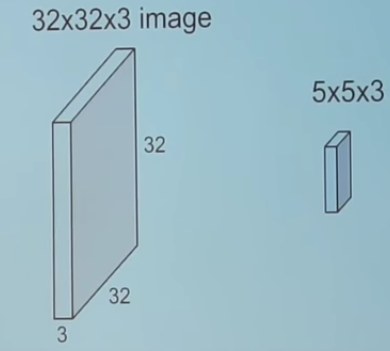
\includegraphics[width=.4\textwidth]{images/Learningprocess/Convolve.png}
    \caption[Convolving an image with a filter]{Convolving an image with a filter}\label{fig: Convolving an image with a filter}%
  \end{figure}
  
We take the 5*5*3 filter and slide it over the complete image and along the way take the dot product between the filter and chunks of the input image.
For every dot product taken, the result is a scalar.
Now, back to CNNs The convolution layer is the main building block of a convolutional neural network.

\begin{figure}[H]%
    \center
	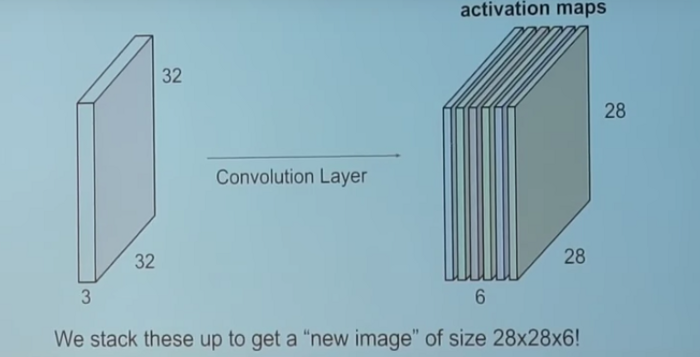
\includegraphics[width=.4\textwidth]{images/Learningprocess/layer.png}
    \caption[Convolution Layer]{Convolution Layer}\label{fig: Convolution Layer}%
\end{figure}
  
 Suppose we have a number of convolution layers in sequence.
 All these filters are initialized randomly and become our parameters which will be learned by the network subsequently.
 
 Take a look at \ref{fig: Filters in a trained network} the filters in the very first layer (these are our 5*5*3 filters). Through back propagation, they have tuned themselves to become blobs of coloured pieces and edges. As we go deeper to other convolution layers, the filters are doing dot products to the input of the previous convolution layers. So, they are taking the smaller coloured pieces or edges and making larger pieces out of them.
 
\ref{fig: Filters in a trained network}. 
\begin{figure}%
    \center
	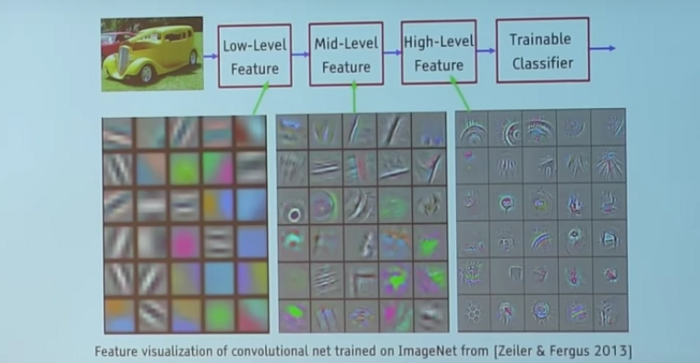
\includegraphics[width=1\textwidth]{images/Learningprocess/nn.png}
	
    \caption[Filters in a trained network]{Filters in a trained network}\label{fig: Filters in a trained network}%
\end{figure}
 
\subsection{Environment}
\subsubsection{World Setup}
\hspace{2cm}The environment composed of a map that satisfies different driving situations and multiple intersections to simulate a real road, the robot-to-map road ratio is the same as the a real car-to-real road ratio as shown in fig \ref{fig: World}. 


\begin{figure}%
\center
    \begin{minipage}[t]{0.3\linewidth}
	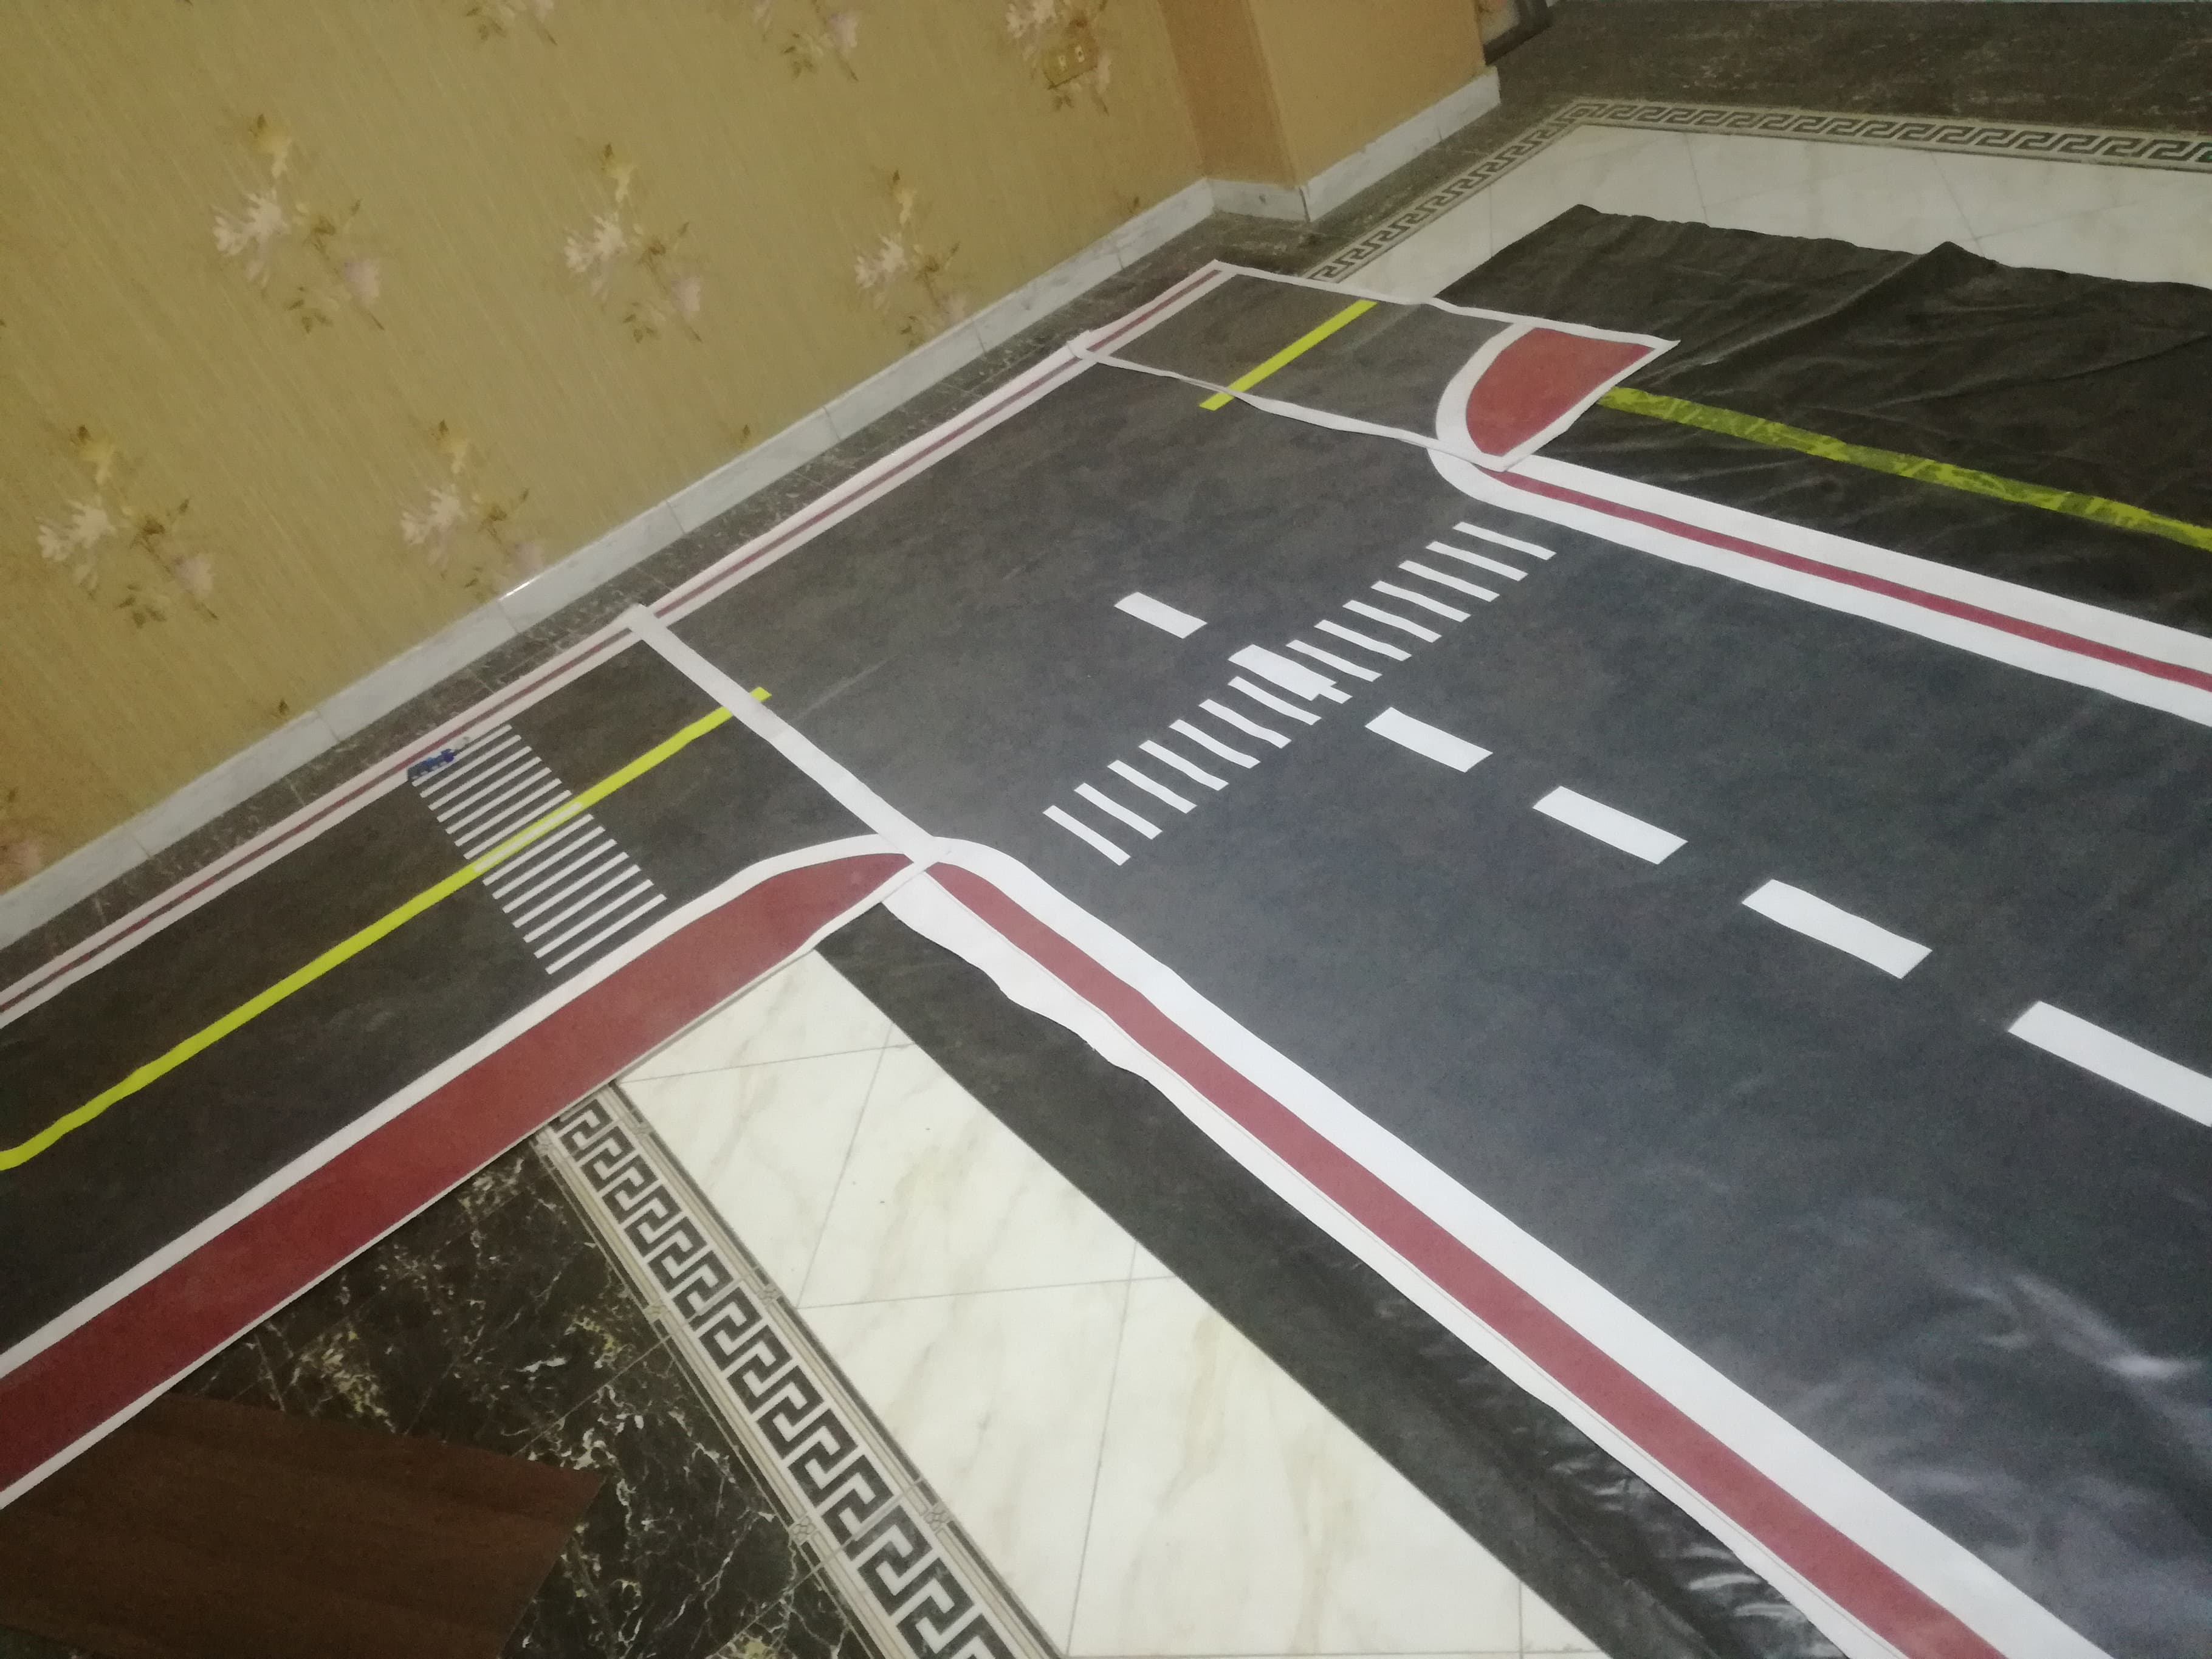
\includegraphics[width=\textwidth]{images/Learningprocess/world2.jpg}
     \end{minipage}
	\begin{minipage}[t]{0.3\linewidth}
	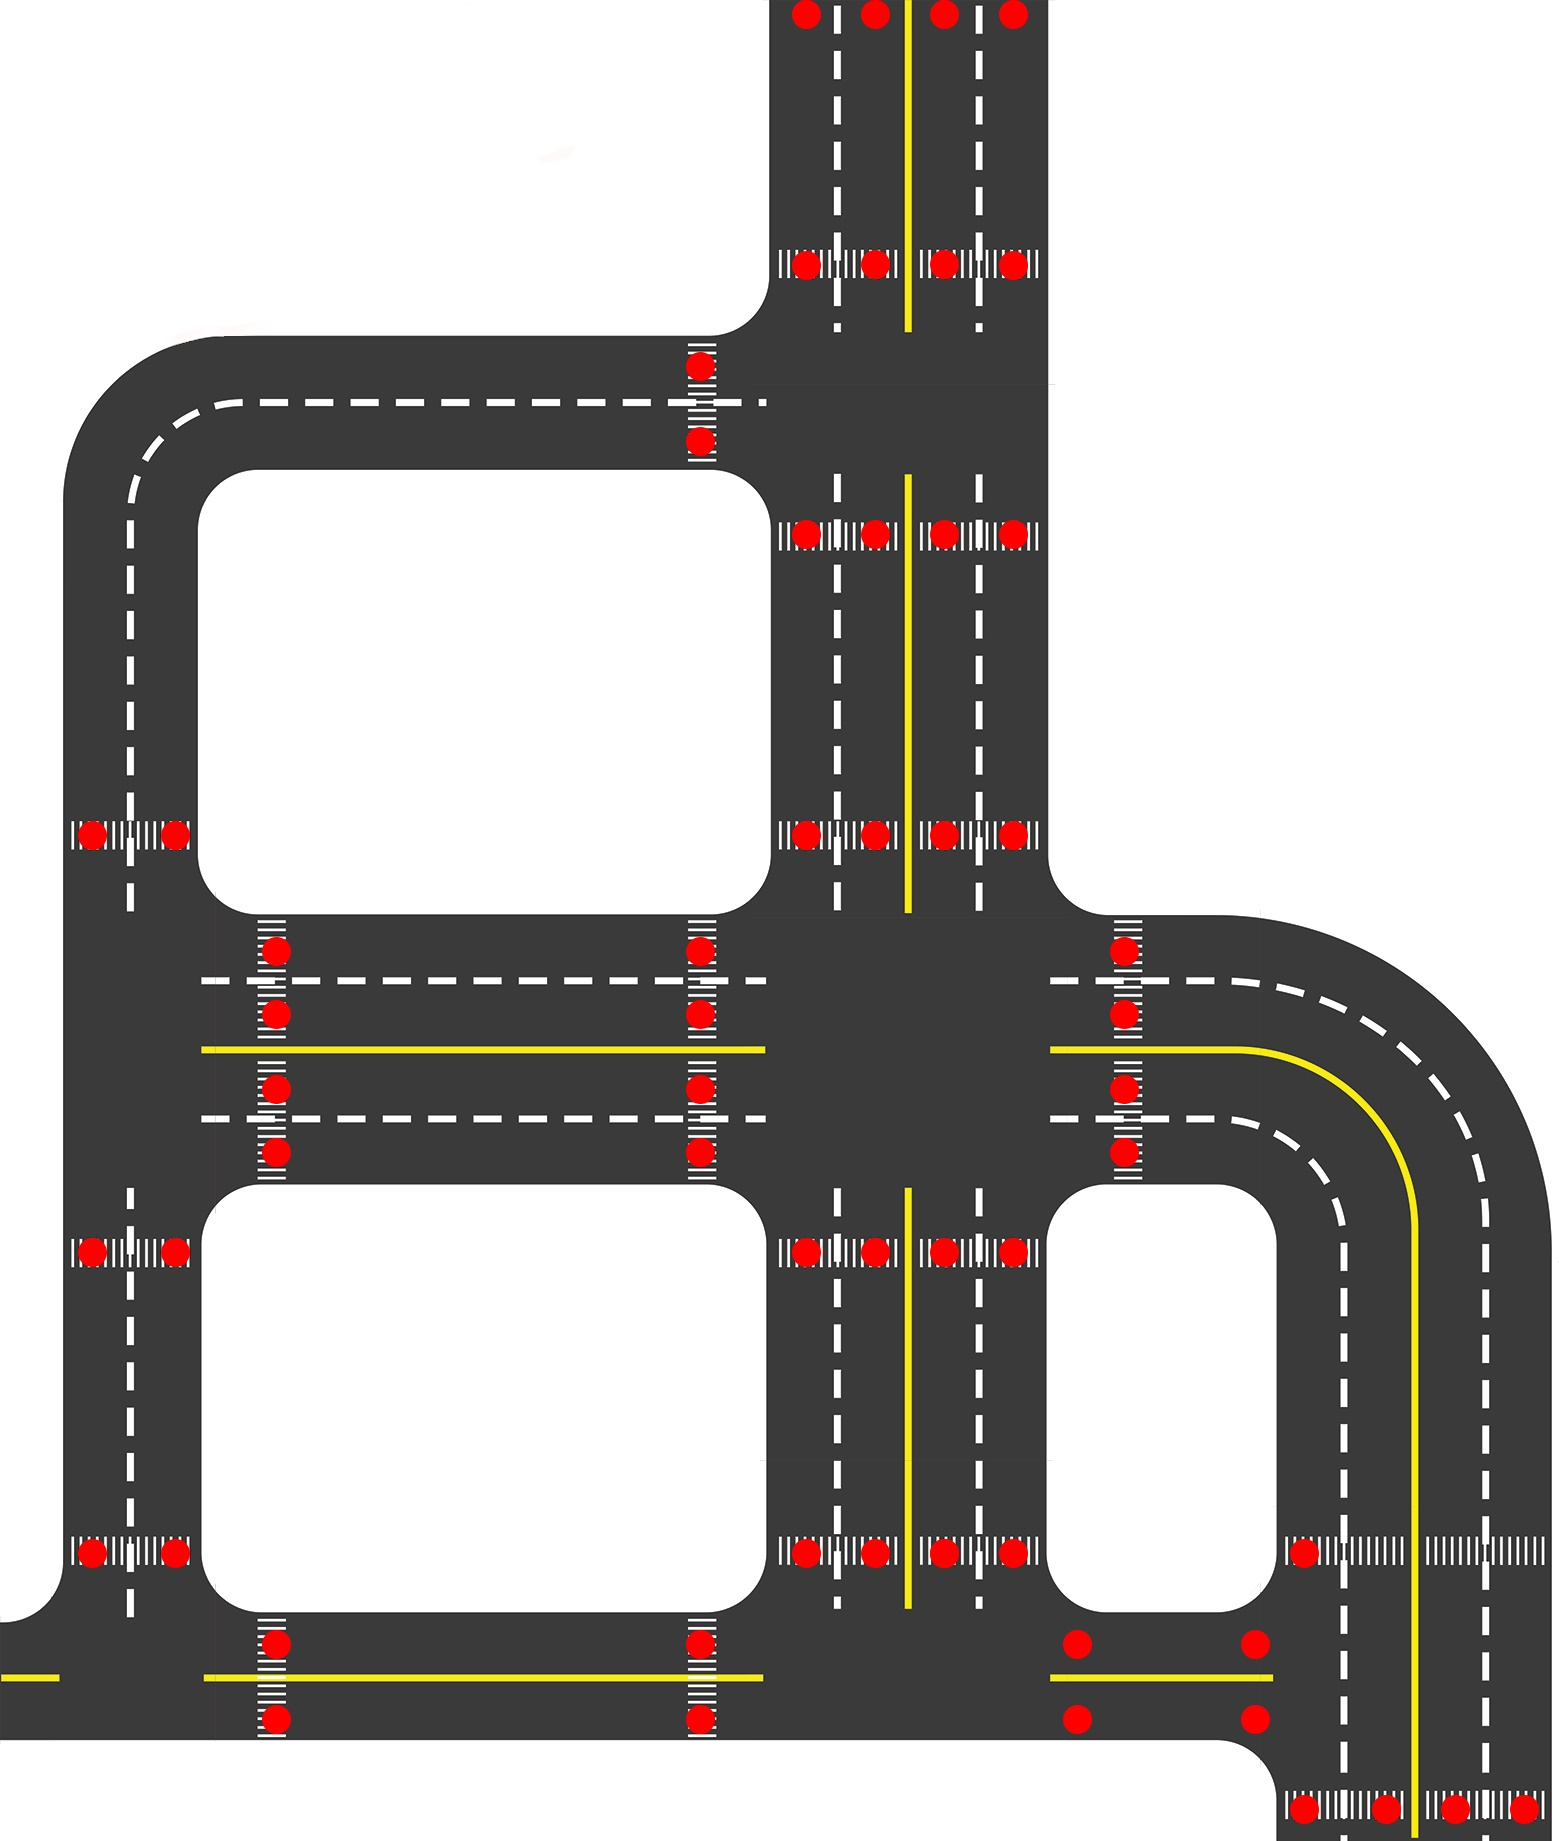
\includegraphics[width=\textwidth]{images/motion/map.jpg}
	\end{minipage}
    \caption[World]{World}\label{fig: World}%
  \end{figure}


\subsubsection{Car Sensors Setup}
\hspace{2cm} Our learning process depends mainly on a RGB Camera to deliver the scene information to The model.
the base of the camera is positioned 14cm in y-axis looking down with 10 degrees angle as shown in fig  \ref{fig: Camera}.

\begin{figure}%
    \center%
    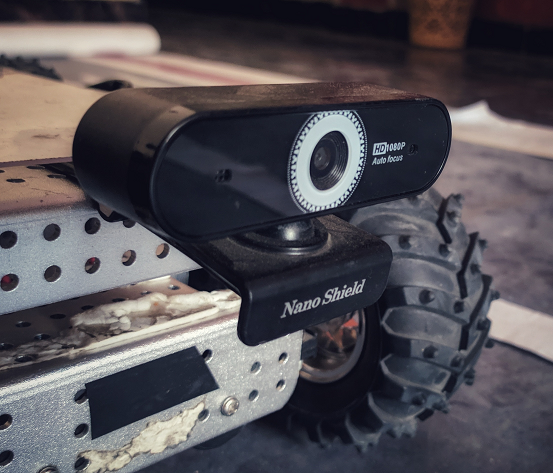
\includegraphics[width=.6\textwidth]{images/Learningprocess/small.png}%
     % you need to add the caption for the list of figures
    \caption[Camera]{Camera}\label{fig: Camera}%
 \end{figure}
 
\subsubsection{Software Environment Setup}
   \hspace{2cm} we use python3-OpenCV package used  for recording and manipulation of the images along side with h5py to save them with extension hdf5.
    we also used keras with back-end tensor-flow==10.13.1 for model construction, training and prediction.
    
\subsubsection{Data Generation}
 \hspace{2cm}During data collection the robot is driven by a human using keyboard and the camera is streaming images, control actions is then synchronized with camera images, then we saved it on the disk image with it's corresponding control actions.
 we started by collecting about 19k images for different scenes and actions in different lights.
 (fig \ref{fig: Data examples})
 
 \begin{figure}%
 \center
 \begin{minipage}[t]{0.3\linewidth}
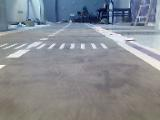
\includegraphics[width=\textwidth]{images/Learningprocess/1.jpg}
 \end{minipage}
\begin{minipage}[t]{0.3\linewidth}
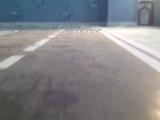
\includegraphics[width=\textwidth]{images/Learningprocess/2.jpg}
\end{minipage}
	\begin{minipage}[t]{0.3\linewidth}
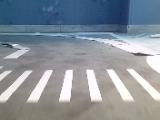
\includegraphics[width=\textwidth]{images/Learningprocess/3.jpg}
\end{minipage}
\begin{minipage}[t]{0.3\linewidth}
    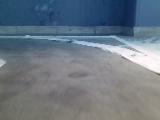
\includegraphics[width=\textwidth]{images/Learningprocess/4.jpg}
\end{minipage}
	\begin{minipage}[t]{0.3\linewidth}
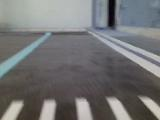
\includegraphics[width=\textwidth]{images/Learningprocess/5.jpg}
\end{minipage}	\begin{minipage}[t]{0.3\linewidth}
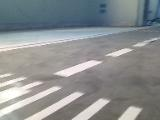
\includegraphics[width=\textwidth]{images/Learningprocess/6.jpg}
\end{minipage}
  \caption[Data examples]{Data examples}\label{fig: Data examples}%
 \end{figure}
\subsubsection{Data Preprocessing}
\begin{enumerate}
    \item For making convergence faster while training the network. Data normalization is done by subtracting the mean from each pixel and then dividing the result by 255.
    \item for the variation and enhancement of the  learning process we start by shuffling all the data with their actions, Shuffling made sure that both train and validation set has data from all different driving conditions like daylight.
    \item for the validation and generalization of the  learning process after the  whole data was shuffled and then split into the train (80\%) and the validation set (20\%)
    \item we defines our ROI by cutting 20 pixels from the top.
    \item the last step was re sizing the images to 120*166.
    (fig \ref{fig: Data preprocessing})
    \begin{figure}%
    \begin{minipage}[t]{0.3\linewidth}
	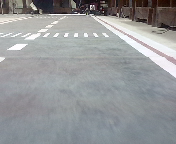
\includegraphics[width=\textwidth]{images/Learningprocess/img3.png}
	\caption[camera photo]{ \left  \newline camera photo}
     \end{minipage}
	\begin{minipage}[t]{0.3\linewidth}
	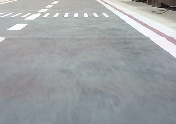
\includegraphics[width=\textwidth]{images/Learningprocess/img4.png}
	\caption[ROI]{ \left \newline ROI}
	\end{minipage}
		\begin{minipage}[t]{0.3\linewidth}
	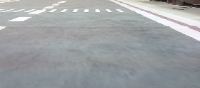
\includegraphics[width=\textwidth]{images/Learningprocess/img2.png}
	\caption[resized Image]{\left \newline \center re-sized Image}
	\end{minipage}
 	\caption[Data preprocessing]{ \center Data preprocessing} \label{fig: Data preprocessing}%
  \end{figure}
\end{enumerate}
\subsection{Data Analysis and Balancing}
\hspace{2cm}During data collection we make sure that data is balanced or not, thi  s could be done by calculating the number of images we took for every possible variation of the data, for example the number of curves, straight lines, cross sections and other possibilities.


\ref{fig: Camera}.
\begin{figure}%
    \center%
    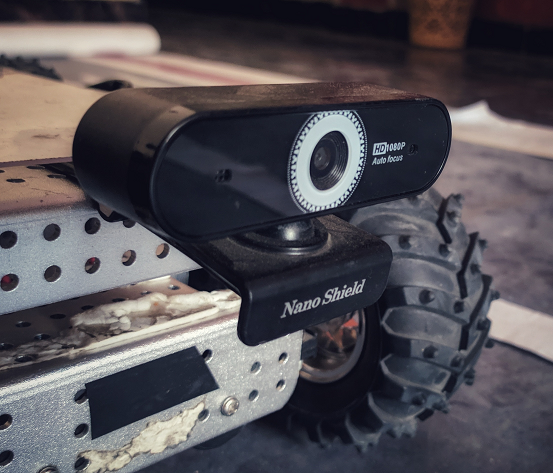
\includegraphics[width=.2\textwidth]{images/Learningprocess/small.png}%
     % you need to add the caption for the list of figures
    \caption[Camera]{Camera}\label{fig: Camera}%
 \end{figure}
\subsection{Neural Network Model}

\subsubsection{Model Architecture}
\hspace{2cm}we picked up two different models for training
    \begin{enumerate}
        \item Donkey car linear model shown in fig \ref{fig: Donkey Car Model Architecture}.
         \item conditional imitation learning model
    \end{enumerate}

\begin{figure}%
    \center%

      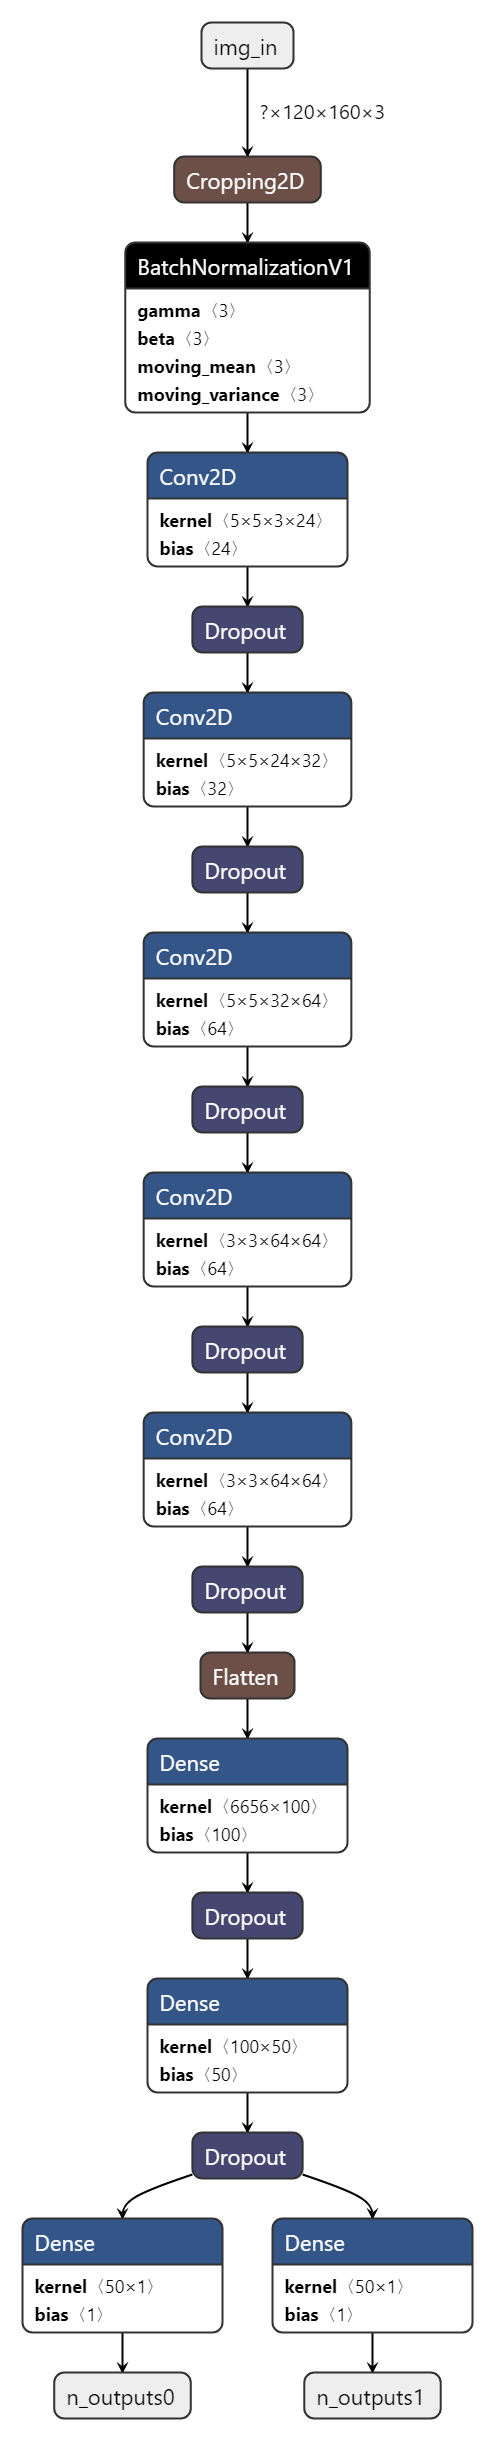
\includegraphics[width=.3\textwidth]{images/Learningprocess/model.png}%
    \caption[Donkey Car Model Architecture]{Donkey Car Model Architecture}\label{fig: Donkey Car Model Architecture}%
 \end{figure}

 \begin{figure}%
  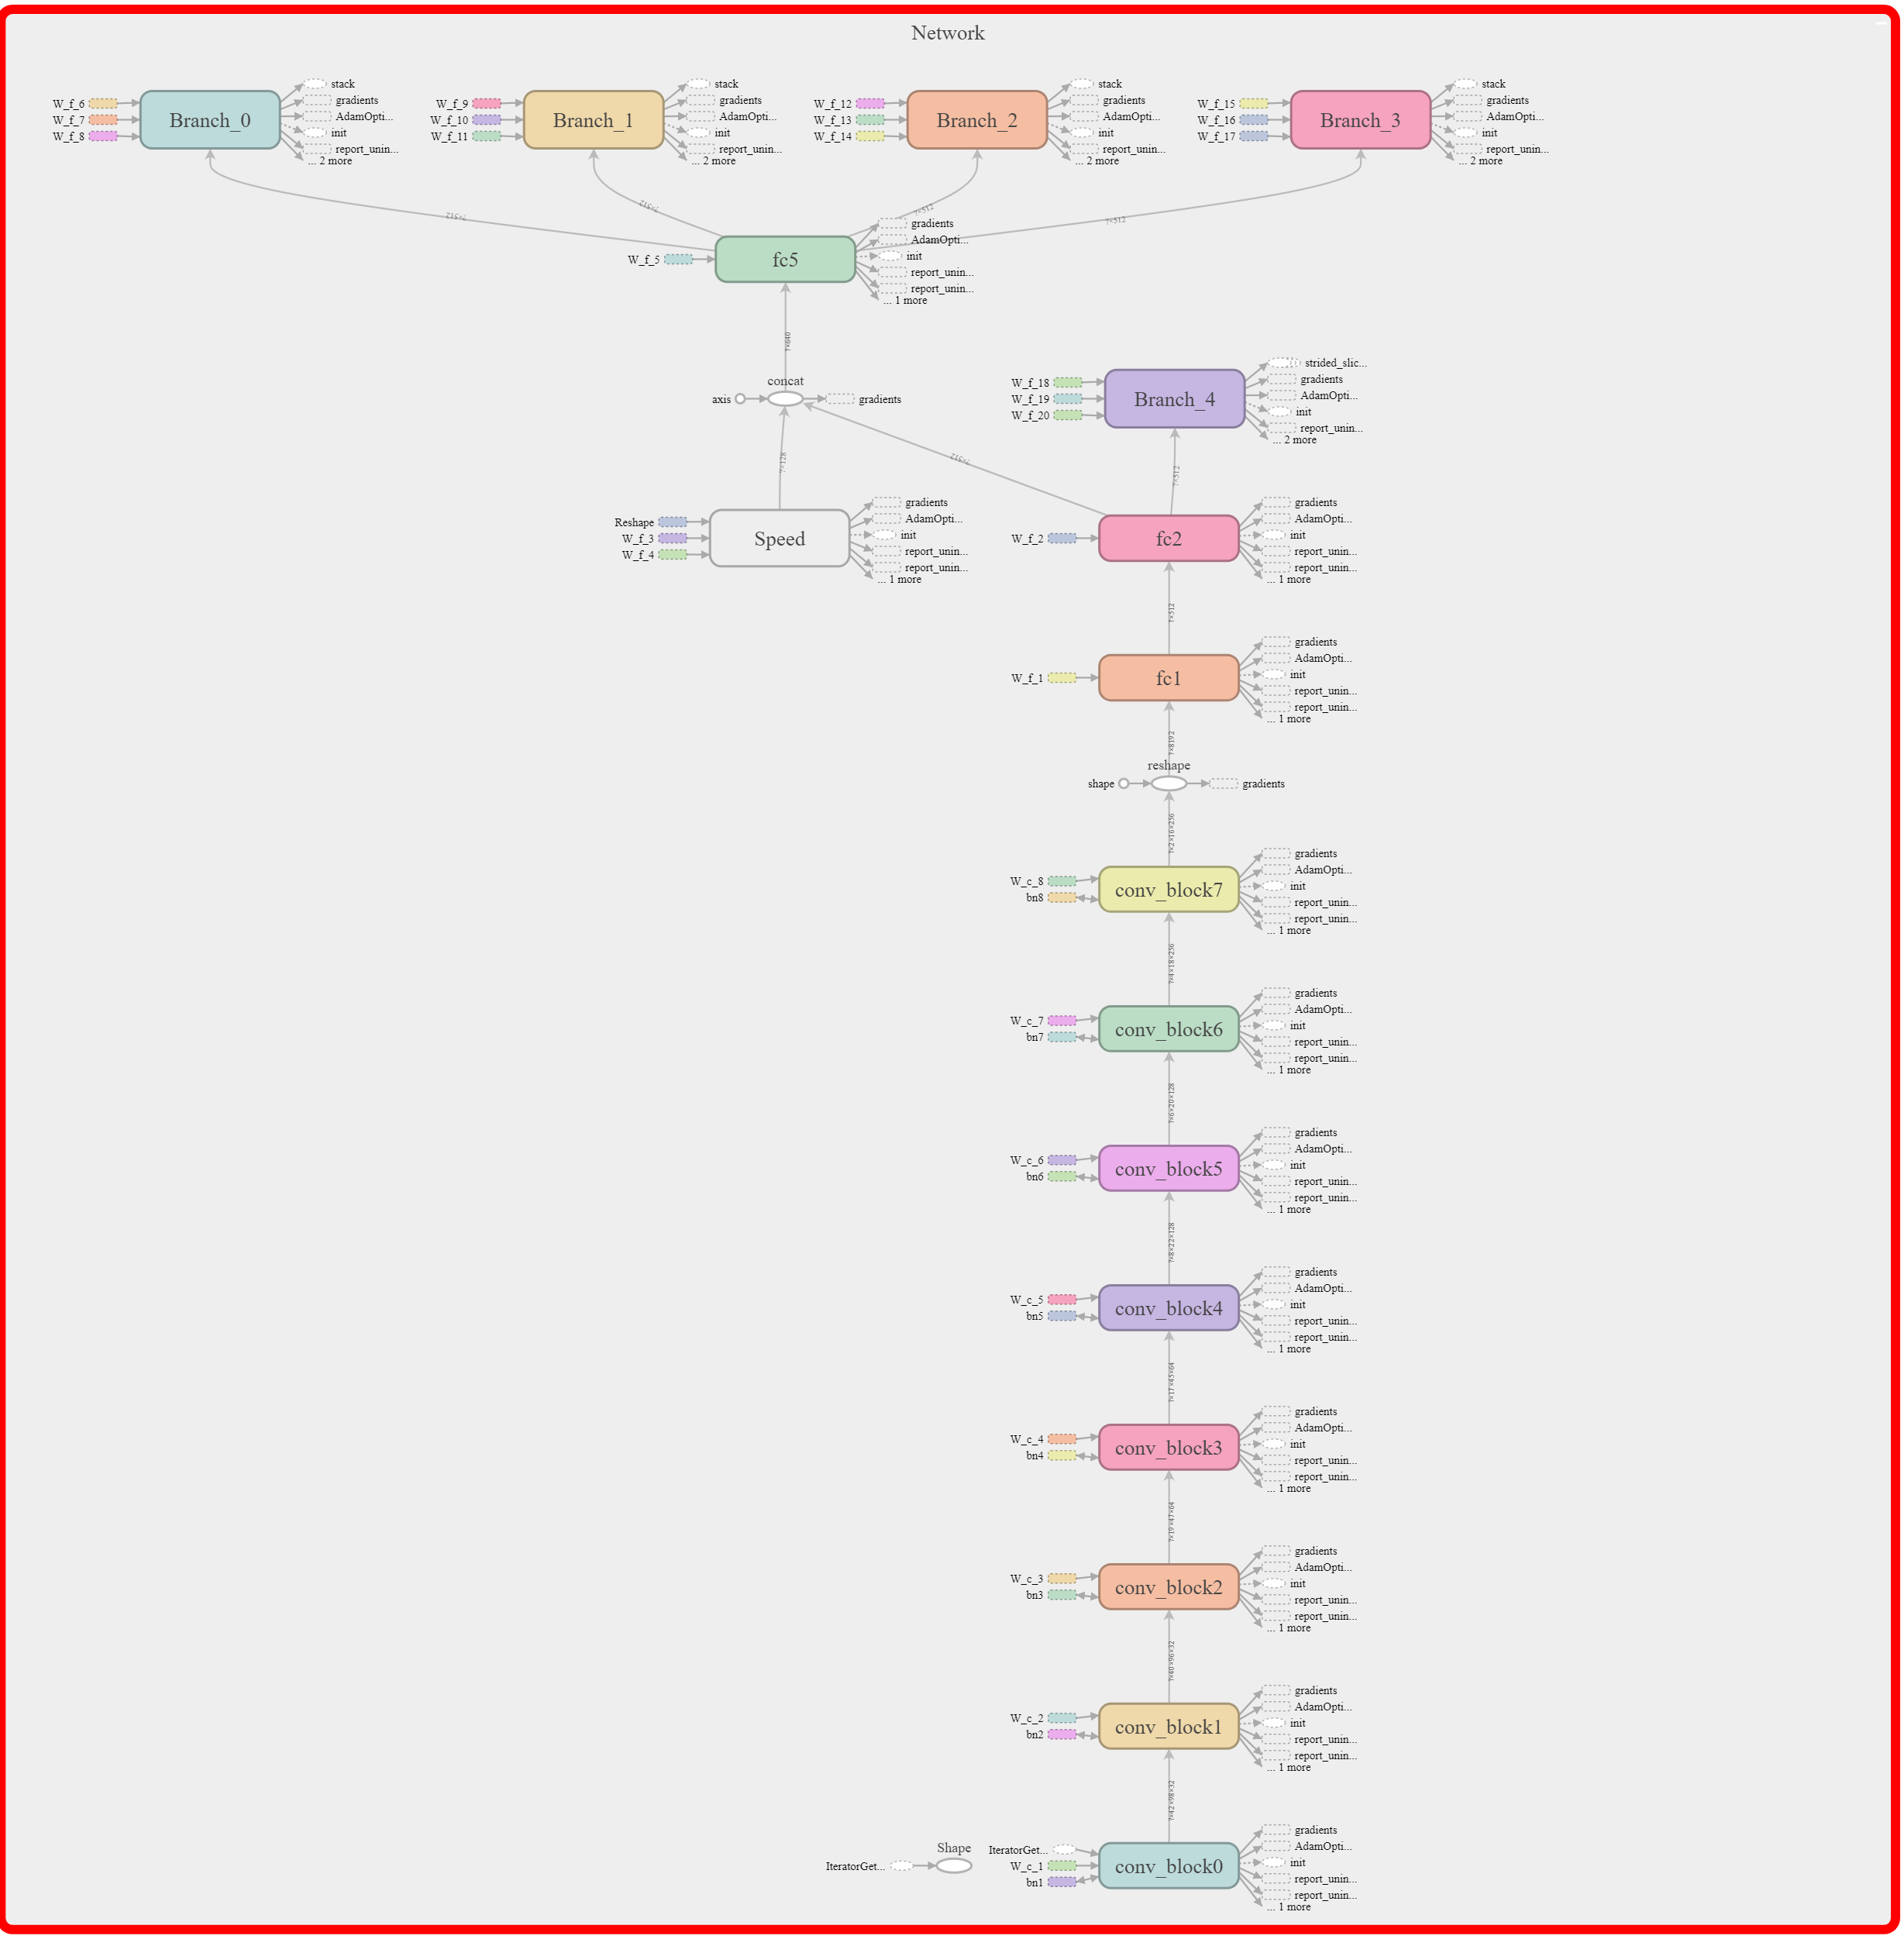
\includegraphics[width=1\textwidth]{images/Learningprocess/carla.png}%
     \caption[conditional imitation learning model]{ conditional imitation learning model}\label{fig:  conditional imitation learning model}%
  \end{figure}
each model have different learning process and architecture resulting in different accuracy, training time and losses.
\subsubsection{Model Training}
\hspace{2cm}when  we started the training process with early step option activated on the donkey car ,the model continued training until reaching 33 epochs of 100  the loss decreased  from loss .8 stepping down until reaching 0.015380 and stopped decreasing subsequently the training.
shown in (fig\ref{5.19}

for conditional imitation learning model training, the model continued training for 100 epochs reaching .001 loss and stopped decreasing.
 \begin{figure}%
 \begin{minipage}[t]{.3\linewidth}
    \center
    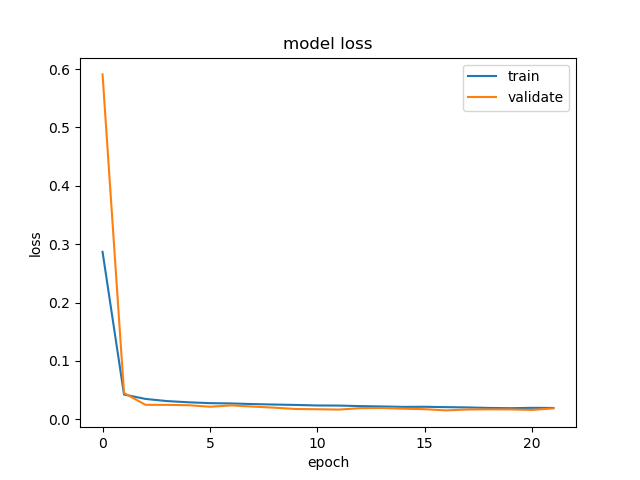
\includegraphics[width=1\textwidth]{images/Learningprocess/lossGraph.png}%

     % you need to add the caption for the list of figures
    \end{minipage}
    \begin{minipage}[t]{.5\linewidth}
    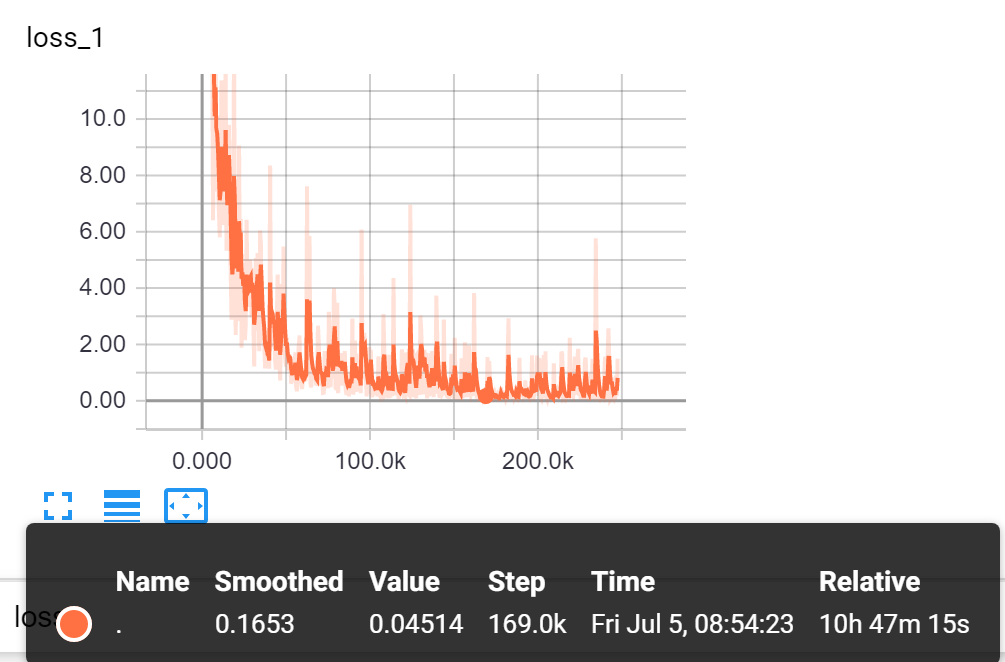
\includegraphics[width=1\textwidth]{images/Learningprocess/carla-valid.png}%
\caption[model losses]{ model losses}\label{fig:  model losses}%
     % you need to add the caption for the list of figures
    \end{minipage}
    
      \end{figure}
\subsubsection{Model Prediction and Output Mapping}

\hspace {2cm}both imitation model and donkey model has achieved good accuracy and low loss after training, the biggest challenge in the process is to run the model on a device that has a good enough requirement that satisfies the running requirements.
for donkey car model prediction we used the raspberry pi 3 b+ for running which achieved reasonable performance with average of 15 frame predicted in second

for imitation learning we used a pc setup with a connected socket with the raspberry bi achieving average of 15 frame predicted in second.
both models has achieved a very good accuracy and low loss.
(fig \ref{fig:  model losses})